\documentclass[conference]{IEEEtran}
\IEEEoverridecommandlockouts
% The preceding line is only needed to identify funding in the first footnote. If that is unneeded, please comment it out.
\usepackage{cite}
\usepackage{amsmath,amssymb,amsfonts}
\usepackage{algorithmic}
\usepackage{graphicx}
\usepackage{textcomp}
\usepackage{xcolor}
\def\BibTeX{{\rm B\kern-.05em{\sc i\kern-.025em b}\kern-.08em
    T\kern-.1667em\lower.7ex\hbox{E}\kern-.125emX}}
\begin{document}

\title{Government AI Readiness Meta-Analysis\\for Latin America and the Caribbean 
%\thanks{Identify applicable funding agency here. If none, delete this.}
}

\author{\IEEEauthorblockN{Laura Montoya}
\IEEEauthorblockA{\textit{Executive Director} \\
\textit{Accel AI}\\
San Francisco, California \\
laura@accel.ai}
\and
\IEEEauthorblockN{Pablo Rivas,~\IEEEmembership{Senior,~IEEE}}
\IEEEauthorblockA{\textit{Department of Computer Science} \\
\textit{Marist College}\\
Poughkeepsie, New York \\
Pablo.Rivas@Marist.edu}
}

\maketitle

% As a general rule, do not put math, special symbols or citations
% in the abstract or keywords.
\begin{abstract}
The abstract goes here.
\end{abstract}

% Note that keywords are not normally used for peerreview papers.
\begin{IEEEkeywords}
IEEE, IEEEtran, journal, \LaTeX, paper, template.
\end{IEEEkeywords}



\section{Introduction}

\IEEEPARstart{E}{ach} country is only as prepared to take advantage of AI technology as it's government and citizens will allow. The US and China, have been leading the competition for the Global AI market, referred to recently as the ``new space race..., where world superpowers battle to define generations of technology to come'' \cite{gershgorn2018ai}. In 2017, China announced a three step plan to become a \$150 billion AI global leader by the year 2030 through investments in research, military, and smart cities. Despite \$10 billion in venture capital currently being funneled towards AI in Silicon Valley, the US has been losing ground, after cutbacks on funding for scientific research and tightening immigration restrictions by the Trump administration, researchers and startups have been opting for grants issued by China to fund the future of AI development \cite{mozur2017china}. But if this is happening in the U.S., then we are inevitably confronted with the question: where does that leave Latin American countries in such Global AI race?

A recent analysis of Government AI readiness, led by Oxford Insights and the International Development Research Centre (IDRC) \cite{miller2019government}, listed no Latin American countries in their top 20 rankings citing three key challenges in harnessing the use of AI for the common good: policies, capacity, and adequate resources. They scored each country and territories governments according to their preparedness to use AI in the delivery of public services. They have stated these findings as ``...a timely reminder of the ongoing inequality around access to AI'' \cite{miller2019government}.

\begin{figure}[!t]
\centering
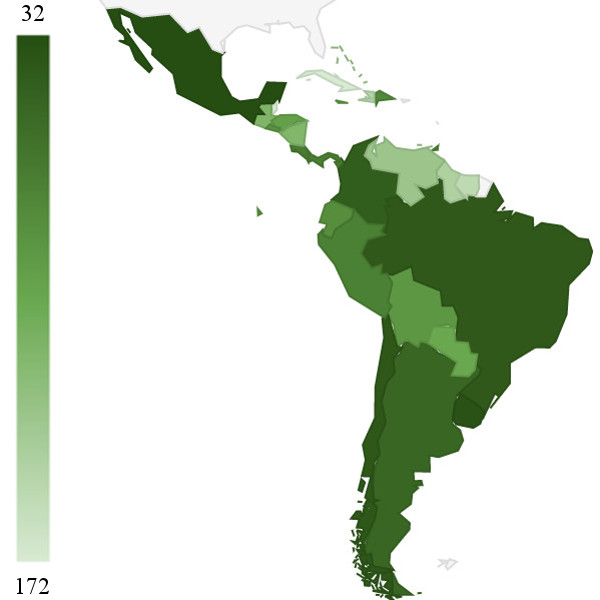
\includegraphics[width=2.5in]{air-rank-no-table}
\caption{Latin American regional comparison geochart produced by LatinX in AI\texttrademark. Data source in \cite{miller2019government}. See Table \ref{tbl:ai-rank} for exact numbers.}
\label{fig:ai-rank}
\end{figure}

\begin{table}[!t]
\caption{Latin American regional comparison by country (first and third column) and AI readiness index (second and fourth column) from data in \cite{miller2019government}.}
\label{tbl:ai-rank}
\centering
\begin{tabular}{|l|l||l|l|}
\hline
Mexico & 32 & Uruguay & 35 \\
Chile & 39 & Brazil & 40 \\
Colombia & 44 & Argentina & 51 \\
Costa Rica & 66 & Panama & 69 \\ 
Peru & 71 & Trinidad and Tobago & 73 \\
Dominican Republic & 77 & Ecuador & 82 \\
El Salvador & 85 & Jamaica & 87 \\     
Bolivia & 89 & Honduras & 96 \\  
Paraguay & 102 & Guatemala & 115 \\    
Nicaragua & 117 & Bahamas & 133 \\     
Venezuela & 134 & Barbados & 135 \\    
Saint Kitts and Nevis & 142 & Dominica & 143 \\
Antigua and Barbuda & 144 & Guyana & 145 \\    
Saint Vincent and the Grenadines & 149 & Haiti & 150 \\
Saint Lucia & 153 & Suriname & 155 \\
Grenada & 164 & Belize & 171 \\
Cuba & 172 & & \\
\hline
\end{tabular}
\end{table}

As can be seen in Fig. \ref{fig:ai-rank} and Table \ref{tbl:ai-rank}, despite not making the top 20, the governments of Mexico, Uruguay, Chile, Brazil, and Colombia ranked within the top 50 countries out of 194 globally. Mexico and Uruguay being the only two South American countries developing AI policies and strategies. Mexico's strategy released in March 2018 \cite{martinho2018mexico}, ``Towards an Artificial Intelligence (AI) Strategy in Mexico: Taking Advantage of the IA Revolution'' was carried out by Oxford Insights, C-Minds, and commissioned by the British Embassy in Mexico. Uruguay opened a public consultation of Artificial Intelligence for the Digital Government on April 22nd, 2019 \cite{uruguay2019inteligencia}, and has since updated its Digital 2020 Agenda \cite{uruguay2019agenda}. However, the rest of Latin American countries still need to make progress to accommodate for the AI revolution.

In this work we present an overview of the key elements contributing to the current status of Latin American AI readiness. First, section X does this...
%% come back to this and finish it after the paper is done.

\section{Overview of The Current Ranking System}

The ranking system created by Oxford and the IDRC, sums an average normalization of indexed metrics on a scale of 0–10, from sources including the UN, WEF, Global Open Data Index, World Bank, Gartner, Nesta, and Crunchbase, clustered under four high-level topics including:
Governance--indicators include whether they had privacy laws in place and a forthcoming AI strategy
Infrastructure and data--indicators include the availability of open sourced data, data capability within the government, and their government's procurement of advanced technology products
Skills and education--indicators include digital skills among the population, innovation capability by the private sector, and the number of registered AI startups
Government and public services--indicators include government effectiveness, availability of digital public services, and the importance of ICTs to government vision of the future
View an index of their data and ranking assessment here.
Comparison table published by LatinX in AI™, Data Source: Government AI Readiness Ranking (0–10 scale) by Oxford Insights and IDRC
The average ranking for Latin American countries according to their analysis is 3.682, not far behind the global average of 4.032. They concluded their analysis stating that ``the way forward is still uncertain'' and suggesting the development of ‘AI Centers' by connecting their academic resources to public and private capital to improve networking and innovation, but also suggesting, until clear and ethical policies for AI have been developed, Latin American governments should heed the warnings of the Latin American Initiative for Open Data, which published a research report titled ``Automating with Caution'' in November 2018.

Examining LATAM AI Readiness Ranking against each Countries Economic Metrics
At first glance, these rankings appear intuitive, but it was surprising to find they did not account for each countries population size, unemployment rate, income equality, household income, education index, or GDP. These metrics are far more telling of a government and it's citizen's ability to invest in or make use of new technology and it's potential effects on the population. I've compared these values to better assess the real risks and potential for integrating artificial intelligence in Latin America.
Unemployment Rate
The unemployment rates, published by the International Monetary Fund, is the number of unemployed persons as a percentage of the total labor force sourced from the World Economic Outlook in 2019. Unemployment in developing countries is often telling of a countries economy but can also be an indicator of factors outside of a government's control. Areas with conflict may see an increase in migration as refugees flee, causing unemployment rates to spike temporarily including in neighboring cities or countries.
Comparison chart by LatinX in AI™, Data sources: Government AI Readiness Index (Oxford \& IDRC), Unemployment Rate (IMF)
This can be seen most clearly in Venezuela, where the unemployment rate has jumped from 6\% in 2015 to 44\% in 2019. ``Venezuela's fall is the single largest economic collapse outside of war in at least 45 years, economists say'', as described in the New York Times and the largest refugee crisis of all time in Latin America. In countries like Venezuela, which used to have a thriving economy largely based on petroleum export and manufacturing, the opportunities for incorporating Artificial Intelligence were endless. Unfortunately now, due to government mismanagement, extensive surveillance and biometric data collection (similar to China's communist regime), coupled with hyperinflation, some say the countries economy may never recover.
This disrupt has even led to some technologically savvy Venezuelan citizens to desperately turn to impersonate US citizen's through virtual private servers (VPS)s' on sites like Mechanical Turk where they end up undermining social science research in order to earn money to feed their families. Venezuelan citizen's fleeing to neighboring countries like Colombia, Argentina, Chile, and Peru, have found opportunities in the local gig economies, working for companies like Rappi, an app based delivery service startup, which is thriving in part due to this influx of migrant workers. Rappi incorporates AI and machine learning techniques in every aspect of their service, their app not only offers food and groceries but also includes on-demand services ranging from personal training to healthcare to even withdrawing and delivering cash from an ATM.
Generally, unemployment rates in a country are a lagging indicator, often following economic distress or improvements and must also be adjusted for seasonal variability. Countries whose economic well-being relies upon a few industries without much room for future development may also show high unemployment rates accompanied by a low GDP per capita. Unemployment and Government AI Readiness are not directly correlated, but unemployment must be considered before implementing AI technology or automation.
Cuba, which has a historically low unemployment rate, also has the lowest Government AI Readiness score out of all other Latin American countries, according to the Oxford and IDRC ratings. Cuba's economy is owned and run by a dictatorship government where the state employ's most of its labor force, sets price standards and controls the access to education, healthcare, and distribution of goods to its citizens. The Cuban government also controls investments in the region, stifling the potential for progress and innovation, although recent economic reforms led by Raúl Castro's administration, have allowed over 400,000 citizens to sign up to be entrepreneurs.
Cuba has also seen an increase in the availability of computers and mobile phones after legalization in 2008, as well as modernization of its telecommunications network, improving access to the internet. As outlined by the Lexington Institute, in their research titled, ``Cuba goes digital'', \$473 million of foreign investment between 1995 and 2000 had given ``Cuba the potential to become a Latin American leader in information technology'' as ``Cuba is incubating a group of enterprises that design and export advanced business and medical software products.'' Anyone knowledgeable about AI technology would know that this could be a great opportunity for incorporating Machine Learning and Deep Learning techniques as solutions for training and deploying models ``on the edge'' through Android and iOS platforms. You can now take advantage of frameworks like TensorFlow Lite by Google, Core ML by Apple, or Caffe2Go by Facebook.
Government acceptance and funding of these technologies for its research institutions and enterprises would have to be sanctioned and appropriately regulated prior to implementation. Government and economic stability would also be needed to warrant investment in the region, unfortunately, large numbers of Cuban citizens have been fleeing the country due to food shortages, impacted by its close ties and oil trade agreements with Venezuela and amplified by travel sanctions imposed by the Trump administration.
GDP PPP
Examining each country's ranking alongside the Gross Domestic Product per Capita Purchasing Power Parity (GDP PPP) will help us to better understand an individual's ability to buy the same quantity of an item in different countries. Government agencies use this metric to compare the output of countries that use different exchange rates and it can be used to forecast future real exchange rates. The GDP PPP is calculated using differences in taxes, tariffs, transportation costs, import costs, and labor costs.
The GDP PPP data, published by the Central Intelligence Agency World Fact Book, compares each countries GDP on a purchasing power parity basis divided by population as of 1 July for the same year.
Comparison chart by LatinX in AI™, Data sources: Government AI Readiness Index (Oxford \& IDRC), GDP-PPP and Population (CIA World Fact Book)
Countries with high GDP PPP may not score highly on this Government AI Readiness index due to having a small population or specialized economy, lacking investment or opportunity for the high impact of technological innovation. This is the case for countries who rely heavily on tourism including Caribbean countries, the Bahamas, Barbados, Antigua and Barbuda, and Saint Kitts.
While some countries with low GDP PPP rank higher on the Government AI Readiness Index thanks in part to a growing or diversified economy combined with technological skills and data protection policies. Ecuador, Peru, Colombia, Brazil, Costa Rica, and the Dominican Republic score above the global average of 4.032 on the Government AI Readiness Index but have historically low GDP PPP.
Ecuador is the 8th largest economy in Latin America with its main industries being petroleum, food processing, textiles, wood products, chemicals —and it is also the world's largest exporter of bananas. At a UN Summit in 2014, Ecuador was one of only five countries who called for a preemptive ban on fully autonomous weapons and in late 2017, in an effort to encourage investment in the region, the National Directorate for the Registration of Public Data in Ecuador (DINARDAP), began drafting the first Ecuadorian law which would implement regulations in order to protect public personal data. Despite these proclamations for privacy and protection, Ecuador has also implemented a nationwide surveillance and response system called ECU 911, funded by China, and making use of controversial facial recognition technology while promoting its benefits for enforcing traffic laws and reducing crime incidents.
Colombia is the 4th largest economy in Latin America, and the fastest growing globally, following China, thanks to its most thriving sectors including construction, services, and agriculture. Its other main industries include textiles, food processing, oil, clothing and footwear, beverages, chemicals, cement, gold, coal, emeralds, shipbuilding, electronics industry, and home appliances. Colombia also has the fastest growing information technology industry in the world and the longest fiber optic network in Latin America, installed by Azteca Co. in 2013.
While Colombia is lacking an official AI strategy, it has some of the most thorough data privacy laws in South America inspired by European data protection regulations. These laws and decrees, enacted between 2008 and 2014, protect its citizens by regulating the use of financial and commercial personal data in credit scoring, they also govern data processing, establish the rights of data subjects and duties of data controllers and processors, set forth requirements for international data transfers, created the National Registry of Databases and designates the Superintendence of Industry and Commerce (SIC) as the data protection authority. In 2018, the first Centre for Excellence in Artificial Intelligence was opened in Medellin, the country's second largest city, as part of the Digital Americas Pipeline Initiative (DAPI), a collaboration between Ruta N, the center of business and innovation of Medellín and IRPA AI (The Institute for Robotic Process Automation and Artificial Intelligence).
An analogy most often used to explain GDP PPP is the Big Mac Index, which compares the price of a Big Mac in different countries in order to illustrate currencies which may be under or overvalued in purchasing power as compared to the local exchange rate. For our purposes, it would be a fruitful undertaking to explore the difference in purchasing power for an AI product and the difference in cost to develop AI across countries, but an in-depth exploration of these questions would merit a write up of its own. We'll use a simple proxy in the interim, the cost to hire AI researchers.
Comparing the Cost to Hire an AI Researcher
The cost to hire an AI Researcher is the most telling comparable metric that governments funding research and development would need to consider in the integration of AI into their policies, products, and services. In the US, salaries of software engineers, data scientists, and researchers skilled in artificial intelligence techniques range between \$100,000–\$150,000 according to PayScale. These averages increase in densely populated or competitive markets like New York and San Francisco. While highly credentialled and ``well-known names in the A.I. field have received compensation in salary and shares in a company's stock that total single- or double-digit millions over a four- or five-year period.''
Alternatively, in Latin America, the cost to hire engineers and researchers is significantly lower ranging between \$15,000 and \$30,000 dependent on years of experience and specialization. According to a 2018 Latin American Developer Survey conducted by Stack Overflow, engineers with some experience in Machine Learning or Data Science still tend to receive higher compensation. Since the job title of Artificial Intelligence engineer and researcher is only beginning to gain popularity, this is the best available historical data to show the average compensation equivalencies by comparison.
Source: ``Hiring Developers in Latin America'' by Julia Silge on Stack Overflow Business Journal
Education
According to the Stack Overflow study, Latin American countries also seem to produce more academic researchers than general software engineers as compared to the rest of the world.
Source: ``Hiring Developers in Latin America'' by Julia Silge on Stack Overflow Business Journal
While the Government AI Readiness Index by Oxford and the IDRC, account for technological skills, they do not look at the overall Education level of a country. The education index is an average of mean years of schooling (of adults) and expected years of schooling (of children), both expressed as an index obtained by scaling with the corresponding maxima. Published by the United Nations Development Program their calculations are developed from data by UNESCO Institute for Statistics (2018) and other sources.
Comparison chart by LatinX in AI™, Data sources: Government AI Readiness Index (Oxford \& IDRC), Education Index (UNDP)
While most Latin American countries rate highly on the education index, many Latin American and Caribbean governments do not invest enough in university research and development. This coupled with unattractive pay, prestige, and working conditions leads to ``Brain Drain'' where the highly skilled or educated leave their country of origin. This phenomenon makes it harder for Universities in those countries to reach their research potential and limits the access to quality scientific research mentors available to share knowledge to incoming students.
A report from Americas Quarterly in 2014 cited data from Mexico's National Council of Science and Technology indicating that 1,271 of the 4,559 Mexicans (28\%) working on master's degrees or Ph.D.s abroad in 2012 were doing so in the US. That's one of every 19 Mexicans with a bachelor's degree or higher living in the US.
In Argentina, scientists often strike to protest budget cuts to research and development. The directors of the National Scientific and Technical Research Council (CONICET), headquartered in Buenos Aires, which employs more than 20,000 researchers in hundreds of centers throughout the country are also fighting the cuts. They created a manifesto demanding ``the immediate implementation of a plan to rescue CONICET.''

Latin American Automation Potential \& Risks
All of these metrics can still only tell part of the story when it comes to a country and it's citizen's preparedness for Artificial Intelligence. You can't predict an economies readiness for AI without including metrics for automation. Several reports have been published in the last five years by experts including the McKinsey Global Institute, the Economist Intelligence Unit, and the International Federation on Robotics, to name a few.
The International Federation of Robotics has been tracking and forecasting the rise of robot density globally for use in manufacturing and affiliated industries. In their 2018 Executive Summary on World Robotics, they noted that Mexico has become an important emerging market for industrial robots outpacing the rest of South America, including Brazil.
International Federation of Robotics--2018 Industrial Robots Executive Summary
The use of AI and automation applied to industries such as manufacturing and agriculture could help to leapfrog a developing countries economy. Countries with a growing young workforce could use these technologies to their advantage in furthering economic development with the right education.
These days, manufacturing with robotics is no longer the largest concern when describing the automation potential and its effects on an economy. Shifts in business processes and software intelligence through automation of data collection and processing will have a larger impact, especially in Latin America. In 2017, the McKinsey Global Institute published its executive summary on ``Harnessing automation for a future that works''.
McKinsey Global Institute--A future that works: Automation, employment, and productivity
They've listed the countries where the potential for automation is highest by adapting current technologies. Of the Latin American countries they included in their study(countries with the largest population or high wages), Peru and Colombia have the highest automation potential at ≥53\%, Brazil, Mexico, and Costa Rica the next highest ≥ 50\% followed closely by Chile, Barbados, and Argentina ≥ 48\%.
McKinsey Global Institute--A future that works: Automation, employment, and productivity
Automation Readiness Index
Meanwhile, the Economist Intelligence Unit developed their own Automation Readiness Index, accompanied by a white paper and executive summary titled ``Who is ready for the coming wave of automation''. Their index, similarly to that of the IDRC and Oxford Insights, categorized metrics under 3 high-level topics including:
Innovation Environment--including indicators for research and innovation, infrastructure, and ethics and safety.
Education Policies--including indicators for basic education, post-compulsory education, continuous education, and learning environments.
Labour Market Policies--including indicators for knowledge on automation and workforce transition programs.
The Economist Intelligence Unit--Automation Readiness Index
They conclude their report by comparing the global use of automation and AI technology to trial and error. Reinforcing the sentiment that ``supporting basic research, clearing the way for start-ups and ensuring competitive markets are likely to be as helpful to AI and robotics innovation as they have been for past technology advances''...while, ``policy directions for education systems and labor markets are less clear for the moment, as the effect of intelligent automation have yet to be widely felt''.
Incorporation of AI into industries through automation which currently relies on a large blue-collar workforce always leads to the concerns of increased unemployment, decreased GPD-PPP, increased migration, and population redistribution or density in city centers, gaps in education for highly technical skills, and increased income inequality between upper and lower class citizens. Most economists say these effects are temporary as the markets shifts and new jobs are developed to support the growth of AI economies, but governments will have to do their part in ensuring their citizens have access to education and opportunities for investment.

How can AI help Latin American Governments and citizens?
Rather than just stressing how AI can be misused by government entities for surveillance to perpetuate bias and corrupt political systems or how it may diminish the middle class and render a country's lower class workers as unemployed, it is important to understand the benefits this technology can add to an ecosystem and economy when used responsibly.
In the public service sector, a myriad of new AI technologies is being implemented including advancing the availability of education, detecting fraud, triaging health care needs, making payments to welfare recipients, speeding immigration decisions, planning and implementation of large urban and industrial infrastructure projects and most importantly, it can reduce costs.
A great write up titled ``The economics of artificial intelligence'' outlines five imperatives for harnessing the power of low-cost prediction, I've paraphrased their descriptions slightly to be applicable to Governments rather than Corporations.
Five Imperatives for Harnessing the Power of Low-Cost Prediction
Develop a thesis on time to AI impact--How fast do I think the implementation, demand, and accuracy of prediction will increase for a particularly valuable AI application in my sector?
Recognize that AI progress will likely be exponential--Once appropriate data collection, processing, and prediction tools are in place for Government services, understand that progress and impact will be exponential rather than linear.
Trust the machines--Where AIs have demonstrated superior performance in prediction, governments must carefully consider the conditions under which to empower humans to exercise their discretion to override the AI.
Know what you want to predict--AI effectiveness is directly tied to goal-specification clarity, so knowing your desired outcomes, whether that be reducing crime rates, increasing the availability of healthcare and education, increasing employment, or reducing government overspending.
Manage the learning loop--Governments need to ensure that information flows into decisions, they follow decisions to an outcome, and then they learn from the outcome and feed that learning back into the system.
The use of AI technology can actually transform the role of governments, making them better able to serve the population. As governments of developing countries continue to shift to more advanced digital platforms, they have added control over the data being collected on their citizens and how that data may be used to benefit society. Since data is the ``new gold'', governments also have a responsibility to their citizens to ensure this information is being mined in the least invasive manner while still creating value for the economy.
In follow-up posts, I'll dive deeper into each Latin American country's economy, current AI research and development in public and private sectors including growth of startups, industrial automation potential, risks, and benefits, that could pave a way forward for LatinX in AI.





\IEEEPARstart{T}{his} demo file is intended to serve as a ``starter file''
for IEEE journal papers produced under \LaTeX\ using
IEEEtran.cls version 1.8b and later.
% You must have at least 2 lines in the paragraph with the drop letter
% (should never be an issue)
I wish you the best of success.

\hfill mds
 
\hfill August 26, 2015

\subsection{Subsection Heading Here}
Subsection text here.

% needed in second column of first page if using \IEEEpubid
%\IEEEpubidadjcol

\subsubsection{Subsubsection Heading Here}
Subsubsection text here.


% An example of a floating figure using the graphicx package.
% Note that \label must occur AFTER (or within) \caption.
% For figures, \caption should occur after the \includegraphics.
% Note that IEEEtran v1.7 and later has special internal code that
% is designed to preserve the operation of \label within \caption
% even when the captionsoff option is in effect. However, because
% of issues like this, it may be the safest practice to put all your
% \label just after \caption rather than within \caption{}.
%
% Reminder: the "draftcls" or "draftclsnofoot", not "draft", class
% option should be used if it is desired that the figures are to be
% displayed while in draft mode.
%
%\begin{figure}[!t]
%\centering
%\includegraphics[width=2.5in]{myfigure}
% where an .eps filename suffix will be assumed under latex, 
% and a .pdf suffix will be assumed for pdflatex; or what has been declared
% via \DeclareGraphicsExtensions.
%\caption{Simulation results for the network.}
%\label{fig_sim}
%\end{figure}

% Note that the IEEE typically puts floats only at the top, even when this
% results in a large percentage of a column being occupied by floats.


% An example of a double column floating figure using two subfigures.
% (The subfig.sty package must be loaded for this to work.)
% The subfigure \label commands are set within each subfloat command,
% and the \label for the overall figure must come after \caption.
% \hfil is used as a separator to get equal spacing.
% Watch out that the combined width of all the subfigures on a 
% line do not exceed the text width or a line break will occur.
%
%\begin{figure*}[!t]
%\centering
%\subfloat[Case I]{\includegraphics[width=2.5in]{box}%
%\label{fig_first_case}}
%\hfil
%\subfloat[Case II]{\includegraphics[width=2.5in]{box}%
%\label{fig_second_case}}
%\caption{Simulation results for the network.}
%\label{fig_sim}
%\end{figure*}
%
% Note that often IEEE papers with subfigures do not employ subfigure
% captions (using the optional argument to \subfloat[]), but instead will
% reference/describe all of them (a), (b), etc., within the main caption.
% Be aware that for subfig.sty to generate the (a), (b), etc., subfigure
% labels, the optional argument to \subfloat must be present. If a
% subcaption is not desired, just leave its contents blank,
% e.g., \subfloat[].


% An example of a floating table. Note that, for IEEE style tables, the
% \caption command should come BEFORE the table and, given that table
% captions serve much like titles, are usually capitalized except for words
% such as a, an, and, as, at, but, by, for, in, nor, of, on, or, the, to
% and up, which are usually not capitalized unless they are the first or
% last word of the caption. Table text will default to \footnotesize as
% the IEEE normally uses this smaller font for tables.
% The \label must come after \caption as always.
%
%\begin{table}[!t]
%% increase table row spacing, adjust to taste
%\renewcommand{\arraystretch}{1.3}
% if using array.sty, it might be a good idea to tweak the value of
% \extrarowheight as needed to properly center the text within the cells
%\caption{An Example of a Table}
%\label{table_example}
%\centering
%% Some packages, such as MDW tools, offer better commands for making tables
%% than the plain LaTeX2e tabular which is used here.
%\begin{tabular}{|c||c|}
%\hline
%One & Two\\
%\hline
%Three & Four\\
%\hline
%\end{tabular}
%\end{table}


% Note that the IEEE does not put floats in the very first column
% - or typically anywhere on the first page for that matter. Also,
% in-text middle ("here") positioning is typically not used, but it
% is allowed and encouraged for Computer Society conferences (but
% not Computer Society journals). Most IEEE journals/conferences use
% top floats exclusively. 
% Note that, LaTeX2e, unlike IEEE journals/conferences, places
% footnotes above bottom floats. This can be corrected via the
% \fnbelowfloat command of the stfloats package.




\section{Conclusion}
The conclusion goes here.





% if have a single appendix:
%\appendix[Proof of the Zonklar Equations]
% or
%\appendix  % for no appendix heading
% do not use \section anymore after \appendix, only \section*
% is possibly needed

% use appendices with more than one appendix
% then use \section to start each appendix
% you must declare a \section before using any
% \subsection or using \label (\appendices by itself
% starts a section numbered zero.)
%


\appendices
\section{Proof of the First Zonklar Equation}
Appendix one text goes here.

% you can choose not to have a title for an appendix
% if you want by leaving the argument blank
\section{}
Appendix two text goes here.


% use section* for acknowledgment
\section*{Acknowledgment}


The authors would like to thank...


\bibliographystyle{IEEEtran}
\bibliography{IEEEabrv,refs}

%\begin{IEEEbiography}[{\includegraphics[width=1in,height=1.25in,clip,keepaspectratio]{mshell}}]{Michael Shell}
% or if you just want to reserve a space for a photo:

\begin{IEEEbiography}{Laura Montoya}
Biography text here.
\end{IEEEbiography}

\begin{IEEEbiography}{Pablo Rivas}
Biography text here.
\end{IEEEbiography}


\end{document}


